\documentclass[conference]{IEEEtran}
\IEEEoverridecommandlockouts
% The preceding line is only needed to identify funding in the first footnote. If that is unneeded, please comment it out.
\usepackage{cite}
\usepackage{amsmath,amssymb,amsfonts}
\usepackage{algorithmic}
\usepackage{graphicx}
\usepackage{textcomp}
\usepackage{xcolor}
\usepackage{tikz}
\usetikzlibrary{arrows.meta,backgrounds,fit,positioning}
\usepackage{url}
\def\BibTeX{{\rm B\kern-.05em{\sc i\kern-.025em b}\kern-.08em
    T\kern-.1667em\lower.7ex\hbox{E}\kern-.125emX}}
\begin{document}

\title{Descubrimiento de Literatura Académica en América Latina: Integración de SciELO y Repositorios Universitarios\\
    %Sistema de recomendación de fuentes académicas: aplicación de embeddings y grafos para de repositorios Latinoamericanos\\
}

\author{
\IEEEauthorblockN{Fabrizzio Marin}
\IEEEauthorblockA{\textit{Departamento de Ingeniería} \\
\textit{Universidad del Pacífico} \\
Lima, Perú \\
sf.marinc@alum.up.edu.pe}
\and\IEEEauthorblockN{Ximena Ramirez}
\IEEEauthorblockA{\textit{Departamento de Ingeniería} \\
\textit{Universidad del Pacífico} \\
Lima, Perú \\
xn.ramirezm@alum.up.edu.pe}
}
\maketitle


% \begin{abstract}
% PROBLEMA
% METODOLOGÍA
% PRINCIPALES HALLAZGOS
% CONCLUSIÓN PRINCIPAL
% de 200 a 250 palabras
% \end{abstract}

% \begin{IEEEkeywords}
% component, formatting, style, styling, insert
% \end{IEEEkeywords}

\section{Introducción}

%%

La revisión de la literatura es clave para delimitar un problema de investigación y sustentar sus decisiones metodológicas, pero el crecimiento y la dispersión de la producción científica dificultan la localización de fuentes pertinentes. La búsqueda manual exige formular muchas consultas en diversas plataformas. Ante ello, los sistemas de recomendación académica emplean técnicas de recuperación de información y representación vectorial para ordenar publicaciones según los intereses del investigador \cite{b1}. En particular, el uso de representaciones semánticas facilita las consultas en lenguaje natural y puede reducir el esfuerzo necesario para encontrar documentos relevantes \cite{b3}.

Los enfoques recientes combinan el contenido textual con información relacional. La integración de embeddings y redes de citación ha mejorado la cobertura y la precisión frente a métodos exclusivamente textuales o estructurales \cite{liu2025llm}. Sin embargo, persisten limitaciones para el contexto latinoamericano: los documentos se distribuyen entre repositorios con estructuras diferentes, los artículos y las tesis rara vez se recuperan de manera conjunta y una lista ordenada de resultados no explica las relaciones temáticas entre las fuentes. Además, buena parte de las herramientas se desarrolla sobre colecciones anglófonas y bases bibliográficas centralizadas \cite{b1}.

Esta limitación es relevante porque el español y el portugués continúan subrepresentados en plataformas académicas anglocéntricas, a pesar de su importancia en las redes regionales de conocimiento \cite{pradier2026}. Los recomendadores pueden reproducir esta desigualdad cuando sus índices y modelos favorecen documentos en inglés o revistas incluidas en bases internacionales \cite{farber2023biases}. En el Perú, esta situación afecta especialmente a las tesis y a otros trabajos depositados en repositorios universitarios, cuyo conocimiento local no siempre aparece en los principales índices bibliográficos. No obstante, las experiencias de acceso abierto muestran que estos documentos pueden integrarse con artículos científicos en sistemas de recomendación multirrepositorio \cite{Borovic2020}.

En respuesta a este vacío, el objetivo del presente trabajo es desarrollar y evaluar un sistema para el descubrimiento de literatura académica latinoamericana que integre artículos de SciELO y tesis de repositorios universitarios peruanos. La hipótesis de trabajo sostiene que la combinación de fuentes heterogéneas, representaciones semánticas multilingües y relaciones documentales ponderadas permitirá recuperar literatura en español de manera más pertinente, diversa y trazable que una búsqueda léxica realizada en un único repositorio.

La metodología se organiza en dos etapas. Primero, se construye un corpus trazable mediante extracción web, normalización y deduplicación, y se comparan TF--IDF, Word2Vec agregado y E5 multilingüe para representar títulos, resúmenes y consultas. Segundo, la consulta original se amplía mediante un modelo de lenguaje de gran tamaño (LLM); posteriormente, los documentos recuperados se exploran a nivel de texto completo y se analizan con LDA, BERTopic y un LLM. A partir de las representaciones del título, el resumen, el contenido y los tópicos, se genera una matriz de adyacencia y un grafo ponderado que permite visualizar la afinidad entre los trabajos.

Las principales contribuciones del estudio son las siguientes:

\begin{itemize}
    \item La integración trazable de artículos y tesis procedentes de repositorios académicos latinoamericanos heterogéneos.
    \item La comparación de representaciones léxicas, distribucionales y semánticas para la recuperación de documentos en español.
    \item Un flujo que vincula recomendación, evidencia del texto completo, identificación de tópicos y construcción de relaciones ponderadas entre documentos.
\end{itemize}

%%

\section{Revisión de Literatura}

Las herramientas de recomendación de fuentes académicas han demostrado su efectividad para hacer el proceso de revisión de literatura más fácil y rápido. Dependiendo de los objetivos, cada solución propuesta aborda problemas como la dispersión de fuentes en diferentes repositorios, evaluación de consultas en lenguaje natural e incorporación de idiomas distintos al inglés \cite{b1}. A continuación se presentan los hallazgos de tendencias clave en la literatura actual sobre el tema.

\textbf{Herramientas de Revisión de Literatura Académica.} Las herramientas actuales para facilitar la revisión de literatura se han beneficiado del desarrollo en técnicas de análisis de datos, lo que ha generado oportunidades y desafíos. Por ejemplo, en ``Scientific paper recommendation systems: a literature review of recent publications'' (2022) \cite{b1}, la abundancia y la variedad de enfoques para desarrollar herramientas de recomendación de papers motivó una revisión de literatura de 65 papers (sobre herramientas de recomendación) de cuatro repositorios diferentes (Google Scholar, ACM DL, dblp y Springer Link) publicados entre enero del 2019 y octubre del 2021. Aplicaron clasificaciones cualitativas para observar la frecuencia de uso de las técnicas más populares. Entre sus resultados, destacamos que los métodos más innovadores no se encuentran disponibles online, se suelen unificar diversas fuentes de datos, y que la audiencia objetivo no suele definirse. También menciona la tendencia de los modelos híbridos (combinando más de una técnica) y la falta de rigurosidad en la evaluación de los modelos, ya sea por benchmark, entre herramientas o por los usuarios mismos. Los autores reconocen la limitación de sus conclusiones al tratarse de un análisis pequeño.

Por el lado aplicativo, ``Scientific Paper Recommendation System: Application of Sentence Transformers and Cosine Similarity Using arXiv Data'' (2025) \cite{b3} aborda la misma problemática anterior: creciente producción académica y dificultad de hallar papers que se ajusten al propósito de cada investigador. Para ello, extrajeron 15 504 papers del repositorio arXiv, en el área de Computer Science. Se aplicó Sentence Transformer (modelo all-MiniLM-L6-v2) y se evaluó la similitud semántica con la métrica similitud coseno. Además, se implementó una interfaz en Streamlit que permite consultas en lenguaje natural por temas/keywords, y se evaluó el rendimiento de su solución con diversas métricas clave y un test de usuario (45 participantes). Así, su propuesta implementa dos factores marcados como puntos de mejora en el paper anterior. El 95.5\% de usuarios estuvieron satisfechos con las recomendaciones y el 93.3\% declaró una reducción significativa del tiempo invertido. Finalmente, entre sus recomendaciones a futuro, sugieren la implementación de un sistema multi-dominio (combinando repositorios).

Por su parte, en ``Academic Literature Recommendation in Large-scale Citation Networks Enhanced by Large Language Models'' (2025) \cite{liu2025llm}, los autores abordan la dificultad de los investigadores para identificar literatura relevante debido a las limitaciones de datos y la sobrecarga de información que enfrentan los métodos tradicionales. Para ello, recolectaron mediante web scraping desde Web of Science un conjunto de 190,381 artículos y 1,087,277 relaciones de citación provenientes de 70 revistas clave en estadística, econometría y ciencias de la computación (1981--2022). Metodológicamente, proponen un marco híbrido que combina la topología de la red de citaciones (vecindad de citas directas e indirectas) con similitud semántica de contenidos, empleando el modelo \textit{text-embedding-3-small} de OpenAI para vectorizar los resúmenes y Bag-of-Words para los títulos, permitiendo ponderaciones flexibles según las preferencias del usuario. En sus resultados, el sistema alcanzó una tasa de acierto promedio del 70\% en la reconstrucción de referencias para artículos de revisión, así como un \textit{hit@1} de 0.85 y un \textit{recall@20} de 0.76 en artículos estándar, demostrando que fusionar la estructura relacional con representaciones semánticas densas mejora sustancialmente la precisión y cobertura frente a enfoques puramente textuales o de grafos.


\textbf{Representación de Fuentes Académicas en Español en la Literatura.} El estudio ``How multilingual is scholarly communication? Mapping the global distribution of languages in publications and citations'' (2026) \cite{pradier2026} indica que el lenguaje genera inequidad en la investigación, estableciendo barreras para los investigadores que no dominan el inglés. Ante ello, buscaron analizar la representación de idiomas en la ciencia, para lo que extrajeron 87,577,942 artículos y 1,480,570,087 referencias citadas de OpenAlex y Dimensions. De sus resultados, se confirma el predominio del inglés, pero también una marcada preferencia intraidioma al citar. Se observa la incorporación gradual de lenguajes como el español y portugués, corrigiendo su subrepresentación en plataformas anglocéntricas, atribuida a una mejora de la indexación.

Dentro de su análisis, este documento indica que Perú produce menos literatura académica en inglés que países como México, Chile o Argentina \cite{pradier2026}. Un análisis limitado a publicaciones en inglés podría subrepresentar la producción científica peruana. Se menciona incluso que en Latinoamérica existen redes de conocimiento regionales en español y portugués ante el aislamiento de la red principal anglocéntrica. 

De manera más específica, ``Biases in scholarly recommender systems: impact, prevalence, and mitigation'' (2023) \cite{farber2023biases} analiza el riesgo de que los sistemas de recomendación académica reproduzcan o amplifiquen sesgos presentes en los datos, los algoritmos y el comportamiento de los usuarios. Su metodología fue una revisión de literatura a partir de búsquedas por palabras clave en Google Scholar, incluyendo también las referencias encontradas (tipo bola de nieve). Analizó 88 documentos sobre sesgos en buscadores o recomendadores académicos y 171 documentos sobre sesgos en sistemas de recomendación en general. Entre los resultados relevantes para este estudio, destaca menor visibilidad para los papers y revistas que no están en inglés y que las citas entre idiomas representan menos del 2\% del total. Además, indican que los usuarios prefieren interactuar con recomendadores presentados en su lengua materna, incluso cuando los documentos sugeridos están escritos en otro idioma.


\textbf{Alcance de Uso de Tesis Académicas.} Si bien la mayoría de las herramientas de recomendación de literatura se enfocan en los papers, las tesis también son una forma de literatura académica válida para incorporar en un sistema de recomendación. El trabajo ``Document Recommendations and Feedback Collection Analysis within the Slovenian Open-Access Infrastructure'' (2020) \cite{Borovic2020} responde a la creciente necesidad de un sistema de recomendación que pueda ayudar a científicos y alumnos, y la gran cantidad de conocimiento no utilizado (las tesis). Para ello, se construyó un sistema de recomendación de fuentes académicas (papers, tesis de pregrado y posgrado, entre otros) multi-repositorio que fomente la colaboración entre investigadores, para implementarlo en la infraestructura Open Access del país (Open Science Slovenia). Su base de datos (al 2020) era el único que abarcaba todos los repositorios de universidades de Eslovenia con todas sus publicaciones electrónicas, teniendo un aproximado de 200,000 documentos que podría recomendar. Su metodología fue aplicar filtrado por contenido y filtrado colaborativo para re-rankear los papers, además de incorporar un flujo constante de nuevos documentos y un módulo de comportamiento del usuario para que vistas, descargas y ratings influyan en las recomendaciones dadas. Como resultado, pudo implementar su ambicioso proyecto e inició un estudio para evaluar sus resultados.

\section{Marco Teórico}

\subsection{Web scraping}

El \textit{web scraping} es el proceso mediante el cual un programa accede a páginas web y extrae parte de su contenido. Cuando una página está escrita en HTML (HyperText Markup Language), su contenido tiene etiquetas que identifican elementos como títulos, párrafos y enlaces. A partir de ello, se puede localizar y almacenar datos específicos \cite{crescenzi2001}. En un repositorio académico, esta información puede incluir el título, los autores, el resumen, las palabras clave y el enlace al documento completo.

\subsection{Representación Vectorial de Textos}

Una forma básica de representar un texto consiste en asignar una dimensión a cada término del vocabulario. Así, un documento puede representarse mediante un vector que indica la presencia o frecuencia de sus palabras, sin considerar el orden en que aparecen. El modelo de espacio vectorial utiliza esta representación para comparar documentos y consultas \cite{salton1975}. Para dar mayor importancia a las palabras que ayudan a distinguir un documento, se puede emplear TF--IDF. La frecuencia de término (TF) representa cuántas veces aparece una palabra en un documento, mientras que la frecuencia inversa de documento (IDF) reduce el peso de las palabras presentes en muchos documentos \cite{sparckjones1972}. Una formulación común es
\begin{equation}
\operatorname{tfidf}(t,d)=\operatorname{tf}(t,d)\log\frac{N}{\operatorname{df}(t)},
\end{equation}
donde $N$ es el número de documentos y $\operatorname{df}(t)$ es la cantidad de documentos que contienen el término $t$. El resultado es una representación útil para identificar coincidencias de palabras, aunque no representa directamente su significado ni el orden en el que aparecen.

Las representaciones densas utilizan vectores de menos dimensiones para aproximar relaciones entre palabras o documentos. Word2Vec propuso las arquitecturas CBOW y \textit{skip-gram}, que aprenden vectores de palabras a partir de los contextos en los que aparecen \cite{mikolov2013}. De esta manera, las palabras utilizadas en contextos parecidos pueden obtener representaciones cercanas. Doc2Vec extendió esta idea mediante un vector que representa un documento completo y que conserva una longitud fija aunque los textos tengan extensiones diferentes \cite{le2014}.

BERT (\textit{Bidirectional Encoder Representations from Transformers}) produce representaciones que consideran el contexto de cada palabra. Durante su preentrenamiento, algunas palabras se ocultan y el modelo aprende a predecirlas utilizando la información que aparece antes y después de ellas \cite{devlin2019}. Por esta razón, una misma palabra puede recibir representaciones diferentes según la oración en la que se encuentre. Estas representaciones pueden adaptarse posteriormente a tareas como clasificación de textos o búsqueda de información.

\subsection{Análisis Semántico}

Una vez representadas una consulta y una fuente académica como vectores, su cercanía puede estimarse mediante la similitud coseno:
\begin{equation}
\operatorname{sim}(\mathbf{q},\mathbf{d})=
\frac{\mathbf{q}\cdot\mathbf{d}}
{\lVert\mathbf{q}\rVert_2\lVert\mathbf{d}\rVert_2}.
\end{equation}
Esta medida compara el ángulo entre los vectores. Un valor mayor indica que la consulta y el documento tienen representaciones más parecidas. En el modelo de espacio vectorial, esta comparación permite ordenar los documentos según su semejanza con una consulta \cite{salton1975}.

El modelado de tópicos busca identificar los temas generales presentes en una colección de textos. La asignación latente de Dirichlet (LDA) representa cada documento como una combinación de tópicos y cada tópico como un conjunto de palabras con diferentes probabilidades \cite{blei2003}. Por ejemplo, un documento puede estar relacionado en distintas proporciones con tópicos como educación, tecnología y economía. Los tópicos se interpretan normalmente observando las palabras a las que el modelo asigna mayor probabilidad.

Los grandes modelos de lenguaje (LLMs por sus siglas en inglés) preentrenados pueden reutilizar el conocimiento adquirido a partir de grandes colecciones de texto para realizar distintas tareas \cite{gpt2}. T5 propuso expresar tareas como clasificación, resumen y respuesta a preguntas mediante un mismo formato: recibir texto como entrada y producir texto como salida \cite{raffel2020}. Bajo este enfoque, la identificación de tópicos puede plantearse como una tarea de clasificación en la que el modelo recibe un documento y devuelve una categoría o etiqueta temática. La calidad de estas etiquetas debe evaluarse con ejemplos de referencia relacionados con el corpus y el idioma del proyecto.

%sugiero
%\subsection{Web scraping}
%párrafo definicion de webscraping y conceptos relacionados (podrias agregar webscraping de papers)

%\subsection{Representación Densa}
%párrafo 1 one-hot-encoding y bag of words (como introduccion) + TF-IDF.

%párrafo 2 word2vec y doc2vec.

%párrafo 3 BERT

%\subsection{Análisis Semántico}
%párrafo 1 Similitud coseno (puedes agregar nociones de distancia l2).

%párrafo 2 topic modelling y LDA Latent Dirichlet Allocation.

%párrafo 3 (Large Language Models como Aprendices Multitarea) hablando sobre como LLMs se usan para tareas de clasificación y/o identificación de tópicos.


\section{Metodología}


%Primero, se realizó la \textbf{recolección de metadatos} mediante \textbf{web scrapping}. Se extrajeron datos de los siguientes repositorios: SciELO, [PENDIENTE] mediante el uso de herramientas como [PENDIENTE]. Así, se obtuvo la siguiente metadata de cada paper: título, revista,[PENDIENTE] y principalmente, el abstract y el enlace al documento en formato .pdf.

%Es importante destacar que el scrapping se realizó como ejercicio académico, debido a la existencia de alternativas como APIs para la descarga.

%Segundo, se aplicó el \textbf{ preprocesamiento} de los datos: quitar los duplicados, corrección de caracteres erróneos, limpieza de stopwords, 

%normalizar? integración título/abstract/keywords?

%Tercero, se realizó la  \textbf{vectorización} de los abstracts utilizando un Sentence Transformer [PENDIENTE, POSIBLEMENTE TF IDF?]. P


%A partir de este punto también se trabajó con una serie de consultas de prueba, que también fueron vectorizadas.
%Acá se supone que decimos tmbn "vectorización de la consulta" pero cómo sería eso? no se supone que es dsps? tipo una vez que ya está todo, recién se hace la prueb
%Antes de esto iría topic omdelling creo? para poder comparar la vectorización de la consulta con la de los abstracts? o me fui mucho?

%Cuarto, se hizo la \textbf{obtención de fuentes más cercanas} mediante el cálculo de la similitud coseno para determinar las k fuentes más cercanos a la consulta evaluada. Con ayuda del metadato de enlace al pdf a la fuente, se extrajeron los archivos completos.

%Quinto, la \textbf{ construcción una red de grafos} donde cada nodo es una fuente y el arista es la relación entre ambos

%acá q? consulta o no? citas o no? se loquea todo, otro embedding o el mismo? (ocr, llm????)

%Finalmente, en la etapa del \textbf{desarrollo de aplicación} se incorporó el proceso de la segunda a la penúltima etapa en un producto funcional, creando una interfaz con la que los usuarios pueden realizar consultas y visualizar las recomendaciones y redes de relaciones entre las fuentes recomendadas.

%En la figura [PENDIENTE] se muestra el flujo de trabajo realizado.

%*gráfico que ha pedido el profe*

%%%
%%%
%%%

Esta sección detalla la metodología desarrollada en el presente trabajo para el descubrimiento y análisis de literatura académica que integra adquisición web, recuperación de información y análisis de relaciones documentales. El sistema emplea SciELO como fuente principal de artículos científicos de América Latina y repositorios de universidades peruanas como fuentes complementarias de tesis y otros trabajos de investigación. Comprende dos etapas. La primera (que se detalla en las subsecciones A y B) construye un corpus trazable de resúmenes, metadatos y enlaces a documentos completos mediante \textit{web scraping}, almacenando los textos y sus representaciones vectoriales. La segunda (que se detalla en las subsecciones C, D y E) se enfoca en recuperar los $K$ abstracts candidatos mejor puntuados para una consulta y sus $N$ subconsultas, procesa los documentos seleccionados e identifica temas y relaciones. Los flujos completos de ambas etapas se resumen en las Figs.~\ref{fig:metodologia-etapa1} y \ref{fig:metodologia-etapa2}, respectivamente. La evaluación compara métodos léxicos, representaciones distribucionales y modelos contextuales, así como procedimientos basados en reglas frente a un modelo de lenguaje de gran tamaño, denominado LLM por sus siglas en inglés. La generación de una discusión y de hipótesis de investigación se considera una extensión opcional.

\subsection{Adquisición y Preparación del Corpus}
\label{subsec:adquisicion}

\subsubsection{Selección de fuentes y criterios de inclusión}

El perfil inicial selecciona publicaciones en español de la colección por País (e.g., Perú) de SciELO, sin restricción de año. La delimitación temática se realiza mediante revistas relacionadas con ingeniería y ciencias (e.g., ingeniería industrial, ecología aplicada, ciencia de datos). Esta selección operativa no equivale a reproducir exactamente las categorías temáticas del buscador central. Se registran las revistas, colecciones y restricciones utilizadas en cada ejecución.

Los repositorios universitarios complementan el corpus con tesis de pregrado, tesis de posgrado y otros trabajos académicos. En cada fuente se identifican las colecciones, facultades o programas de interés, y se registran el idioma y el periodo de publicación. La incorporación posterior de otras bases académicas reutiliza el mismo procedimiento mediante adaptadores específicos de navegación y extracción. La inclusión en el índice inicial requiere un título, una URL de procedencia y un abstract utilizable en español. El idioma de la interfaz no sustituye al idioma de publicación.

\subsubsection{Herramientas y estrategia de rastreo}

La adquisición se realiza mediante solicitudes HTTP y análisis de páginas HTML, sin utilizar APIs de metadatos. El componente de SciELO emplea Python, \texttt{requests} para recuperar las páginas y \texttt{BeautifulSoup} para parsear y analizar su estructura. Los adaptadores universitarios aplican reglas de navegación y selectores adecuados a cada repositorio, manteniendo un esquema común de salida.

%En SciELO, el descubrimiento sigue la secuencia catálogo de revistas, números publicados y artículos. En los repositorios se recorren colecciones, listados paginados y fichas documentales. Los enlaces relativos se resuelven respecto de la página de origen y se incorporan a una cola persistente. Para cada URL se conserva la página desde la cual fue descubierta, permitiendo reconstruir el recorrido de adquisición.

Las solicitudes incluyen pausas, tiempos de espera y reintentos limitados. Se registran estados HTTP, redirecciones y errores de análisis. La cola distingue documentos pendientes, procesados, filtrados y no recuperados, de modo que una ejecución interrumpida pueda reanudarse. Las respuestas de bloqueo o error no se contabilizan como documentos válidos.

\subsubsection{Extracción de información documental}

Para cada artículo o tesis se conserva el HTML de la ficha o página principal y se recuperan los campos publicados por la fuente. El esquema documental incluye identificador de origen, URL, título, autores, fecha, idioma, revista o institución, tipo de documento, abstract y enlaces a PDF y/o XML. También se extraen DOI, identificadores persistentes y palabras clave cuando estén disponibles.

% puede generar tabla para hacer un diccionario de datos de lo que se menciona arriba

En SciELO se conservan adicionalmente las etiquetas de metadatos, los enlaces y los datos estructurados incluidos en el HTML. Si existen resúmenes en varios idiomas, se preservan sus versiones y se selecciona la versión en español para el perfil inicial. 

%La captura del HTML corresponde al cuerpo de la respuesta y no implica descargar automáticamente imágenes, hojas de estilo o recursos ejecutados mediante JavaScript. Asimismo, un enlace PDF o XML encontrado indica disponibilidad anunciada, no una descarga realizada ni una validación del archivo. Esta distinción permite separar la recolección inicial de metadatos del procesamiento posterior del texto completo.

\subsubsection{Preprocesamiento y control de calidad}

El preprocesamiento elimina etiquetas HTML de los campos textuales y normaliza espacios, saltos de línea y códigos de idioma. El resumen se separa de menús, encabezados, palabras clave y otras secciones de la página. 

%La validación comprueba la presencia de campos mínimos, el idioma seleccionado, la unicidad del registro y la integridad del HTML almacenado. Se contabilizan campos ausentes, exclusiones y errores por fuente. Estas comprobaciones evalúan la consistencia técnica de la adquisición; no miden por sí mismas la relevancia temática ni la cobertura exhaustiva de los repositorios.

\subsubsection{Identidad documental y deduplicación}

Cada registro utiliza una clave interna estable, \texttt{paper\_id}, compartida por la base de metadatos y los índices de búsqueda. Se conservan por separado los identificadores externos, como DOI, PID de SciELO o identificador persistente del repositorio. El DOI no se utiliza como única clave porque puede estar ausente.

El control de duplicados dentro de SciELO utiliza la fuente y el identificador del artículo. Los adaptadores universitarios mantienen un espacio de identificación propio de cada fuente. Para la integración entre repositorios se contempla una clave adicional, \texttt{work\_id}, que agrupe versiones confirmadas de una misma obra, conservando sus registros de procedencia. 

\subsubsection{Almacenamiento y trazabilidad}

El componente de SciELO almacena registros y estados de procesamiento en SQLite y permite exportarlos en JSONL. El HTML original se conserva comprimido, junto con la URL, la fecha de recuperación y una huella de integridad. Los adaptadores adicionales se integran mediante el esquema documental común, preservando los atributos específicos de cada repositorio.

La arquitectura separa metadatos, archivos e índices. El índice de resúmenes vincula cada vector con \texttt{paper\_id}. Los archivos se identifican mediante \texttt{file\_id} y su huella; los fragmentos del texto completo incorporan \texttt{chunk\_id}, \texttt{paper\_id} y \texttt{file\_id}. Para cada representación se registran el modelo, su revisión, la configuración y la versión del texto. Una modificación de estos componentes exige actualizar los vectores afectados.


%%%
%%%
%%%

\subsection{Representación de Abstracts}
\label{subsec:representacion}

Sea $\mathcal{D}=\{p_1,\ldots,p_N\}$ el corpus documental. Para cada abstract $p_i$ se construye un texto $x_i$ mediante la concatenación de título y resumen. Las palabras clave podrán añadirse como una variante controlada, utilizando la misma información de entrada para todos los métodos comparados. Se evaluarán tres representaciones: TF-IDF, Word2Vec agregado y BERT.

\subsubsection{Representación léxica mediante TF-IDF}

Esta técnica representa cada texto mediante un vector disperso de términos ponderados según su frecuencia en el documento y su frecuencia inversa en el corpus. El vocabulario y las ponderaciones se ajustan una vez sobre el corpus de indexación. Las consultas se transforman con ese mismo modelo, sin reajustarlo con cada búsqueda.

\subsubsection{Representación mediante Word2Vec}

A diferencia de TF-IDF, nos proporciona vectores de palabras, por lo que requiere una operación de agregación para representar resúmenes y consultas. Se utilizará un promedio ponderado por TF-IDF:
\begin{equation}
 \mathbf{u}(x)=
 \frac{\sum_{t\in V_x}w(t,x)\mathbf{e}_t}
 {\sum_{t\in V_x}w(t,x)},
 \label{eq:word2vec}
\end{equation}
donde $V_x$ contiene los términos con representación disponible, $w(t,x)$ es su peso TF-IDF y $\mathbf{e}_t$ el vector de la palabra. El resultado de \eqref{eq:word2vec} se normaliza antes de la recuperación.

\subsubsection{Representación mediante BERT}

La representación densa contextual de los abstracts se obtendrá mediante un modelo BERT multilingüe (\texttt{intfloat/multilingual-e5-base}) preentrenado \cite{wang2024}. Cada abstract se tokeniza en subpalabras y se procesa con BERT para generar representaciones contextualizadas. Estas se agregan mediante el promedio de los vectores de la última capa, excluyendo los tokens especiales y de relleno, y el vector resultante se normaliza con la norma $L_2$. Las consultas se codifican con el mismo modelo y el mismo procedimiento de agregación para que puedan compararse con los abstracts mediante similitud coseno.

Cada abstract se representa como una unidad cuando cabe en la ventana de entrada de BERT. Cuando supera el límite de tokens del modelo, se segmenta por oraciones en fragmentos que respetan dicho límite. Los vectores de los fragmentos se combinan mediante un promedio ponderado por su cantidad de tokens y se normalizan nuevamente, de modo que cada abstract conserve una única representación en el índice. El índice del texto completo conservará, en cambio, un vector por fragmento.

\subsubsection{Índices de búsqueda y escalabilidad}

La similitud entre la consulta $q$ y el documento $p$ se calcula mediante:
\begin{equation}
 s(q,p)=
 \frac{\mathbf{v}_q^{\mathsf T}\mathbf{v}_p}
 {\|\mathbf{v}_q\|_2\|\mathbf{v}_p\|_2}.
 \label{eq:coseno}
\end{equation}
Con vectores normalizados, \eqref{eq:coseno} equivale al producto interno. El sistema ordena los documentos por esta puntuación y recupera los primeros $k$. La puntuación se interpreta como proximidad representacional, no como probabilidad de relevancia.

% FIGURA ETAPA 1 (A--B)
\begin{figure*}[!t]
\centering
\resizebox{\textwidth}{!}{%
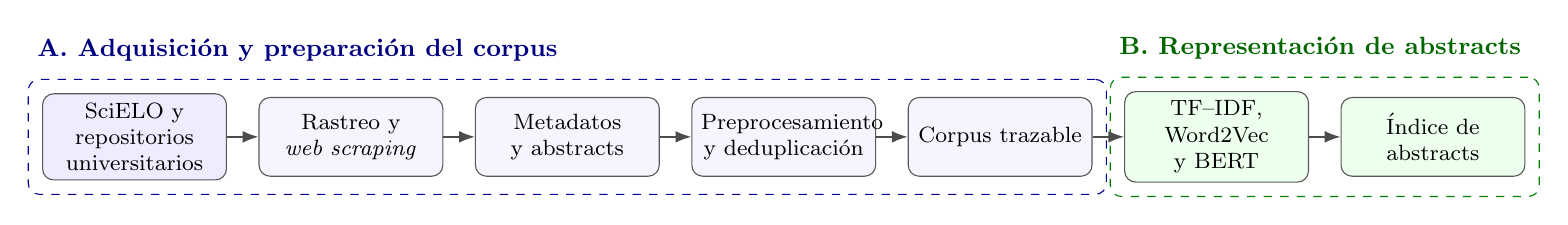
\begin{tikzpicture}[
box/.style={draw=black!65,rounded corners,minimum height=10mm,text width=2.1cm,align=center,font=\footnotesize,fill=white},
arr/.style={->,semithick,draw=black!70},node distance=4mm,>=Latex]
\node[box,fill=blue!7] (f) {SciELO y repositorios universitarios};
\node[box,fill=blue!4,right=of f] (r) {Rastreo y \textit{web scraping}};
\node[box,fill=blue!4,right=of r] (e) {Metadatos y abstracts};
\node[box,fill=blue!4,right=of e] (q) {Preprocesamiento y deduplicación};
\node[box,fill=blue!4,right=of q] (c) {Corpus trazable};
\node[box,fill=green!7,right=of c] (v) {TF--IDF, Word2Vec y BERT};
\node[box,fill=green!7,right=of v] (i) {Índice de abstracts};
\foreach \a/\b in {f/r,r/e,e/q,q/c,c/v,v/i}{\draw[arr] (\a)--(\b);}
\begin{scope}[on background layer]
\node[draw=blue!60!black,dashed,rounded corners,fit=(f)(c),inner sep=5pt] (ab) {};
\node[draw=green!50!black,dashed,rounded corners,fit=(v)(i),inner sep=5pt] (bb) {};
\end{scope}
\node[above=1mm of ab.north west,anchor=south west,font=\small\bfseries,text=blue!50!black] {A. Adquisición y preparación del corpus};
\node[above=1mm of bb.north west,anchor=south west,font=\small\bfseries,text=green!40!black] {B. Representación de abstracts};
\end{tikzpicture}}
\caption{Flujo metodológico de la Etapa 1: construcción del corpus y del índice de abstracts.}
\label{fig:metodologia-etapa1}
\end{figure*}


%%%
%%%
%%%

\subsection{Recomendación de Literatura}
\label{subsec:consultas}

\subsubsection{Consulta original y subconsultas}

Se define un método que recupera los $K$ abstracts mejor puntuados para la consulta $q_0$. Para mejorar el funcionamiento de esta búsqueda, a partir de la consulta original, un LLM genera $N$ subconsultas (se fija $N=3$, con subconsultas $q_1,q_2,q_3$) que preservan el objetivo y desarrollan facetas complementarias. Las salidas contienen identificador, descripción de la faceta y texto de búsqueda. Se conservan las instrucciones, el modelo y la consulta original para reproducir el procedimiento.

Por ejemplo, para una consulta sobre simulación social y dinámica de opiniones mediante agentes basados en modelos de lenguaje, las facetas pueden abordar la implementación de agentes, los mecanismos de cambio de opinión y la evaluación de las dinámicas simuladas. Las facetas exploratorias no se convierten automáticamente en requisitos de inclusión. Se evita introducir autores, resultados o restricciones no solicitados y se mantienen visibles las reformulaciones para su revisión.

Las subconsultas se generan una sola vez para cada consulta y se reutilizan entre los métodos de representación. Esta decisión permite atribuir diferencias a la recuperación y no a variaciones de las reformulaciones producidas por el LLM.

\subsubsection{Selección sin reranking}

El modo exploratorio recupera cinco resultados para cada consulta y consolida el conjunto:
\begin{equation}
 \mathcal{C}(q_0)=
 \bigcup_{j=0}^{N}\operatorname{Top}_{K}(q_j),
 \qquad |\mathcal{C}(q_0)|\leq{(N+1)K}.
 \label{eq:candidatos}
\end{equation}
La unión de \eqref{eq:candidatos} puede contener menos de veinte documentos por solapamiento. Cada documento conserva las consultas que lo recuperaron, sus posiciones y puntuaciones, pero se descarga una sola vez (más detalles en la siguiente sección).

\subsection{Exploración de literatura}
\label{subsec:exploracion}

\subsubsection{Descarga del documento y extracción de texto}

Los candidatos se vinculan con sus metadatos mediante \texttt{paper\_id}; a partir de ese registro se obtiene el enlace al PDF. Para la descarga se desarrolla un script de \textit{web scraping} para obtener el documento, que comprueba el formato del archivo y registra URL final, estado, huella y fecha. Se reutilizan archivos previamente recuperados cuando su versión coincide. Las páginas de error no se procesan como documentos científicos.

Se extraerá primero el texto nativo con PyMuPDF. El reconocimiento óptico de caracteres (OCR) se aplicará únicamente a páginas sin texto utilizable o con extracción defectuosa, utilizando los idiomas necesarios. Se comprobarán problemas de orden de lectura, columnas y encabezados repetidos. La aplicación de OCR quedará registrada por página, pues sus errores pueden afectar la recuperación y la interpretación de resultados.

Los documentos no accesibles conservarán sus metadatos y su resultado basado en el resumen. Un fallo de descarga no se interpretará como irrelevancia. Los experimentos con texto completo utilizarán el mismo subconjunto accesible para los métodos comparados y reportarán por separado la cobertura alcanzada.

\subsubsection{Segmentación y vinculación con el documento original}

El texto se segmentará respetando secciones y párrafos cuando puedan identificarse. Se establece como punto de partida un máximo de 300 tokens de contenido por fragmento y un solapamiento de hasta 40 tokens. Se reservará espacio para título, sección y prefijos dentro de la ventana del codificador. Estos valores se consideran parámetros experimentales y podrán ajustarse exclusivamente con los datos de desarrollo.

Cada fragmento conservará identificador, documento, archivo, sección, páginas y texto original. Se almacenarán offsets y coordenadas de los bloques cuando estén disponibles, junto con el mapeo hacia la versión normalizada. Esta vinculación permitirá localizar las frases utilizadas por el sistema y resaltarlas en el PDF. Las referencias bibliográficas se conservarán en un campo separado para analizar citas sin confundirlas con aportes propios del documento.

\subsubsection{Recuperación de fragmentos relevantes}

Los fragmentos se representarán con el mismo codificador denso y se almacenarán en un índice separado del índice de abstracts. Para cada par consulta--documento se recuperarán hasta tres fragmentos no redundantes mediante \eqref{eq:coseno}. La búsqueda se restringirá al identificador documental correspondiente para evitar que un trabajo extenso monopolice la evidencia del conjunto.

% FIGURA ETAPA 2 (C--E)
\begin{figure*}[!t]
\centering
\resizebox{0.75\textwidth}{!}{%
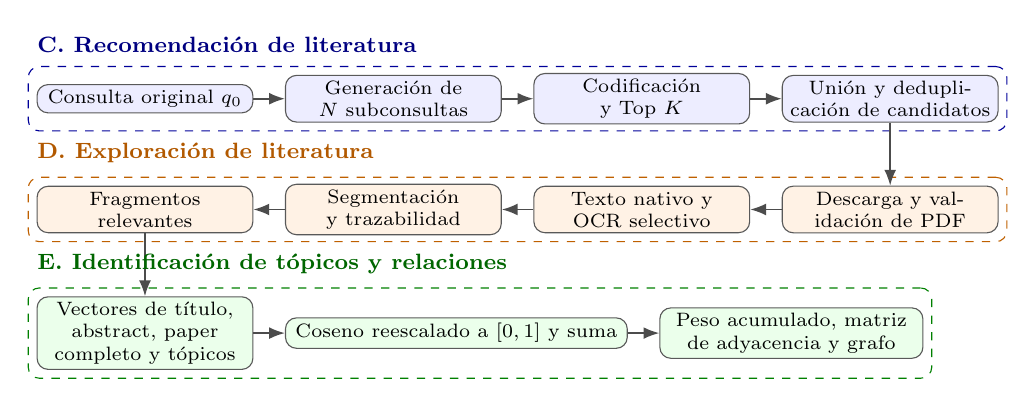
\begin{tikzpicture}[
box/.style={draw=black!65,rounded corners,minimum height=3mm,text width=2.6cm,align=center,font=\scriptsize,fill=white,inner sep=2pt},
arr/.style={->,semithick,draw=black!70},node distance=4mm,>=Latex]
\node[box,fill=blue!7] (q0) {Consulta original $q_0$};
\node[box,fill=blue!7,right=of q0] (qs) {Generación de $N$ subconsultas};
\node[box,fill=blue!7,right=of qs] (tk) {Codificación y Top $K$};
\node[box,fill=blue!7,right=of tk] (ca) {Unión y deduplicación de candidatos};
\node[box,fill=orange!10,below=8mm of ca] (pdf) {Descarga y validación de PDF};
\node[box,fill=orange!10,left=of pdf] (ocr) {Texto nativo y OCR selectivo};
\node[box,fill=orange!10,left=of ocr] (seg) {Segmentación y trazabilidad};
\node[box,fill=orange!10,left=of seg] (fr) {Fragmentos relevantes};
\node[box,fill=green!8,below=8mm of fr] (ut) {Vectores de título, abstract, paper completo y tópicos};
\node[box,fill=green!8,right=of ut,text width=4.2cm] (mt) {Coseno reescalado a $[0,1]$ y suma};
\node[box,fill=green!8,right=of mt,text width=3.2cm] (out) {Peso acumulado, matriz de adyacencia y grafo};
\foreach \a/\b in {q0/qs,qs/tk,tk/ca,ca/pdf,pdf/ocr,ocr/seg,seg/fr,fr/ut,ut/mt,mt/out}{\draw[arr] (\a)--(\b);}
\begin{scope}[on background layer]
\node[draw=blue!60!black,dashed,rounded corners,fit=(q0)(ca),inner sep=3pt] (cc) {};
\node[draw=orange!75!black,dashed,rounded corners,fit=(fr)(pdf),inner sep=3pt] (dd) {};
\node[draw=green!50!black,dashed,rounded corners,fit=(ut)(out),inner sep=3pt] (ee) {};
\end{scope}
\node[above=.5mm of cc.north west,anchor=south west,font=\footnotesize\bfseries,text=blue!50!black] {C. Recomendación de literatura};
\node[above=.5mm of dd.north west,anchor=south west,font=\footnotesize\bfseries,text=orange!70!black] {D. Exploración de literatura};
\node[above=.5mm of ee.north west,anchor=south west,font=\footnotesize\bfseries,text=green!40!black] {E. Identificación de tópicos y relaciones};
\end{tikzpicture}}
\caption{Flujo metodológico de la Etapa 2: recomendación, exploración, identificación de tópicos y construcción del grafo ponderado de relaciones.}
\label{fig:metodologia-etapa2}
\end{figure*}


%%%
%%%
%%%


\subsection{Identificación de Tópicos y Relaciones}
\label{subsec:relaciones}

\subsubsection{Modelado temático mediante LDA}

Se empleará Latent Dirichlet Allocation (LDA) como método estadístico de referencia. A partir de conteos de palabras, LDA estima una distribución de tópicos por documento y una distribución de palabras por tópico \cite{blei2003}. El ajuste se realizará sobre un corpus de referencia fijado antes de procesar las consultas de prueba. Se evaluarán distintos números de tópicos y semillas mediante coherencia, diversidad y estabilidad. 


\subsubsection{Modelado temático mediante BERTopic}

BERTopic es un modelo de tópicos que extrae representaciones temáticas coherentes mediante el desarrollo de una variante de TF-IDF basada en clases \cite{bertopic}. Más concretamente, BERTopic genera representaciones vectoriales de documentos utilizando modelos de lenguaje basados en \textit{transformers} previamente entrenados, agrupa dichas representaciones y, finalmente, genera representaciones de los temas mediante el procedimiento TF-IDF basado en clases. BERTopic genera temas coherentes y mantiene un rendimiento competitivo frente a diversos modelos de referencia, tanto clásicos como aquellos que siguen el enfoque de agrupamiento más reciente para el modelado de temas.

\subsubsection{Extracción temática mediante LLM}

El LLM analizará las mismas unidades textuales utilizadas en la comparación temática y generará una salida estructurada con temas, términos representativos y pasajes de apoyo. Se fijará un procedimiento de normalización de etiquetas y consolidación de sinónimos, construido con los datos de desarrollo. La cantidad de temas y el presupuesto de texto se documentarán para evitar ventajas atribuibles a diferencias de entrada.

\subsubsection{Construcción de la matriz de adyacencia y el grafo}

Para representar las relaciones entre los papers se conservarán por separado cuatro representaciones vectoriales para cada paper $p_i$: el título $\mathbf{h}_i$, el abstract $\mathbf{a}_i$, el contenido completo $\mathbf{d}_i$ y la información temática $\mathbf{t}_i$. El título y el abstract se codificarán con el mismo modelo denso utilizado en la recuperación. La representación del contenido completo se obtendrá agregando los vectores de sus fragmentos, mientras que la representación temática procederá de LDA, BERTopic y/o el LLM.

La similitud coseno convencional toma valores en el intervalo $[-1,1]$. Para evitar cancelaciones entre componentes positivos y negativos, cada valor se transformará al intervalo $[0,1]$ mediante
\begin{equation}
\operatorname{sim}_{01}(\mathbf{x},\mathbf{y})=
\frac{1+\operatorname{sim}(\mathbf{x},\mathbf{y})}{2}.
\label{eq:coseno-reescalado}
\end{equation}
Cuando se utilice más de un método temático, la similitud temática $s_{ij}^{(t)}$ será el promedio de las similitudes reescaladas obtenidas por los métodos seleccionados, por lo que también permanecerá en $[0,1]$. El peso compuesto entre dos papers será la suma directa de los cuatro componentes:
\begin{equation}
w_{ij}=
\operatorname{sim}_{01}(\mathbf{h}_i,\mathbf{h}_j)
+\operatorname{sim}_{01}(\mathbf{a}_i,\mathbf{a}_j)
+\operatorname{sim}_{01}(\mathbf{d}_i,\mathbf{d}_j)
+s_{ij}^{(t)}.
\label{eq:peso-compuesto}
\end{equation}
La matriz de adyacencia $\mathbf{A}\in\mathbb{R}^{M\times M}$ se construirá como
\begin{equation}
A_{ij}=
\begin{cases}
w_{ij}, & i\neq j,\\
0, & i=j.
\end{cases}
\label{eq:adyacencia}
\end{equation}
El peso $w_{ij}$ queda acotado entre $0$ y $4$: un valor cercano a $4$ indica una alta afinidad conjunta, mientras que un valor cercano a $0$ indica una relación débil en las cuatro representaciones. La matriz es simétrica y representa un grafo ponderado no dirigido: cada nodo corresponde a un paper y cada arista utiliza $w_{ij}$ como peso. Las filas, columnas y nodos conservarán el mismo \texttt{paper\_id} utilizado en los índices. Para garantizar pesos comparables, el análisis principal utilizará el subconjunto de papers que cuente con las cuatro representaciones; los documentos sin texto completo conservarán sus resultados basados en título y abstract, pero se reportarán por separado. Para la visualización podrán ocultarse las aristas con pesos bajos sin modificar la matriz completa almacenada.



\begin{thebibliography}{00}
\bibitem{b1}
C. K. Kreutz and R. Schenkel,
``Scientific paper recommendation systems: A literature review of recent publications,''
\textit{International Journal on Digital Libraries}, vol. 23, pp. 335--369, 2022.
\url{https://doi.org/10.1007/s00799-022-00339-w}

\bibitem{b3}
A. P. Putra, D. P. S. Putri, and A. K. A. C. Wiranatha,
``Scientific paper recommendation system: Application of sentence transformers and cosine similarity using arXiv data,''
\textit{Journal of Applied Informatics and Computing (JAIC)}, vol. 9, no. 4, pp. 1374--1382, 2025.
\url{https://api.semanticscholar.org/CorpusID:281123317}

\bibitem{pradier2026}
C. Pradier, L. Céspedes, and V. Larivière,
``How multilingual is scholarly communication? Mapping the global distribution of languages in publications and citations,''
\textit{Journal of the Association for Information Science and Technology}, vol. 77, no. 5, pp. 699--713, 2026.
\url{https://doi.org/10.1002/asi.70055}

\bibitem{farber2023biases}
M. Färber, M. Coutinho, and S. Yuan,
``Biases in scholarly recommender systems: Impact, prevalence, and mitigation,''
\textit{Scientometrics}, vol. 128, pp. 2703--2736, 2023.
\url{https://doi.org/10.1007/s11192-023-04636-2}

\bibitem{Borovic2020}
M. Borovič, M. Ferme, J. Brezovnik, S. Majninger, K. Kac, and M. Ojsteršek,
``Document recommendations and feedback collection analysis within the Slovenian open-access infrastructure,''
\textit{Information}, vol. 11, p. 497, 2020.

\bibitem{liu2025llm}
K. Liu, Y. Zhang, R. Pan, \textit{et al.},
``Academic literature recommendation in large-scale citation networks enhanced by large language models,''
\textit{Scientometrics}, vol. 130, pp. 5143--5169, 2025.
\url{https://doi.org/10.1007/s11192-025-05420-0}



%%%%lo de abajo ya es marco teorico

\bibitem{crescenzi2001}
V. Crescenzi, G. Mecca, and P. Merialdo,
``RoadRunner: Towards automatic data extraction from large Web sites,''
in \textit{Proc. 27th Int. Conf. Very Large Data Bases (VLDB)}, 2001,
pp. 109--118.


\bibitem{sparckjones1972}
K. Spärck Jones,
``A statistical interpretation of term specificity and its application in retrieval,''
\textit{Journal of Documentation}, vol. 28, no. 1, pp. 11--21, 1972.
\url{https://doi.org/10.1108/eb026526}

\bibitem{salton1975}
G. Salton, A. Wong, and C. S. Yang,
``A vector space model for automatic indexing,''
\textit{Communications of the ACM}, vol. 18, no. 11, pp. 613--620, 1975.
\url{https://doi.org/10.1145/361219.361220}

\bibitem{mikolov2013}
T. Mikolov, K. Chen, G. Corrado, and J. Dean,
``Efficient estimation of word representations in vector space,''
in \textit{Proc. 1st Int. Conf. Learning Representations (ICLR)}, 2013.
\url{https://arxiv.org/abs/1301.3781}

\bibitem{le2014}
Q. Le and T. Mikolov,
``Distributed representations of sentences and documents,''
in \textit{Proc. 31st Int. Conf. Machine Learning}, vol. 32, 2014,
pp. 1188--1196.
\url{https://proceedings.mlr.press/v32/le14.html}

\bibitem{devlin2019}
J. Devlin, M.-W. Chang, K. Lee, and K. Toutanova,
``BERT: Pre-training of deep bidirectional transformers for language understanding,''
in \textit{Proc. 2019 Conf. North American Chapter of the Association for Computational Linguistics: Human Language Technologies}, 2019,
pp. 4171--4186.
\url{https://doi.org/10.18653/v1/N19-1423}

\bibitem{wang2024}
L. Wang, N. Yang, X. Huang, L. Yang, R. Majumder, and F. Wei,
``Multilingual E5 text embeddings: A technical report,''
\textit{arXiv preprint arXiv:2402.05672}, 2024.
\url{https://arxiv.org/abs/2402.05672}

\bibitem{gpt2}
A. Radford, J. Wu, R. Child, D. Luan, D. Amodei, and I. Sutskever,
``Language models are unsupervised multitask learners,''
OpenAI, Tech. Rep., 2019.
\url{https://cdn.openai.com/better-language-models/language_models_are_unsupervised_multitask_learners.pdf}


\bibitem{blei2003}
D. M. Blei, A. Y. Ng, and M. I. Jordan,
``Latent Dirichlet allocation,''
\textit{Journal of Machine Learning Research}, vol. 3, pp. 993--1022, 2003.
\url{https://www.jmlr.org/papers/v3/blei03a.html}

\bibitem{bertopic}
M. Grootendorst,
``BERTopic: Neural topic modeling with a class-based TF-IDF procedure,''
\textit{arXiv preprint arXiv:2203.05794}, 2022.
\url{https://arxiv.org/abs/2203.05794}

\bibitem{raffel2020}
C. Raffel \textit{et al.},
``Exploring the limits of transfer learning with a unified text-to-text transformer,''
\textit{Journal of Machine Learning Research}, vol. 21, no. 140, pp. 1--67, 2020.
\url{https://www.jmlr.org/papers/v21/20-074.html}

\end{thebibliography}
\end{document}
